% -*- LaTeX -*-

\part{Case studies}

\chapter{Introduction}
Several studies in which the \vamps\ model has been used are
presented in the following chapters. It is hoped that this
not only gives a good idea about \vamps{}' capabilities, but
will also help the user when working with the program.
To give an idea of the
possible uses of vamps I will shortly describe three (semi-realistic)
cases and how \vamps\ can cope with these cases:
\begin{enumerate}
\item
A small lysimeter located in west Java, Indonesia worked most of the
time. However discharge data from several days is
missing. Transpiration, interception en soil-evaporation fluxes are
already calculated (and measured) by other means. In this case \vamps\
is used to estimate the discharge for the missing days.
To simulate the lysimeter as accurate as possible \vamps\ is
used with a no flow bottom boundary and lateral flow allowed
only on the bottom soil node.
\item
Fiji \ldots
\end{enumerate}


%\chapter{Three forest types in the Luquillo Mountains}
%\section{Introduction}
%\section{The palm forest}
%\section{The Tabonuco forest}
%\section{The elfin forest}

\chapter{A {\em Pinus caribaea} plantation forest}\label{chap:fiji}
\section{Introduction}
This chapter shows the results of running \vamps\ on a dataset
concerning a {\em Pinus caribaea} plantation forest, located on Viti
Levu, Fiji (see~\citeasnoun{waterloo1994T2}). A 61 days period (July 2
-- September 2) from the Tulasewa site was modeled using
meteorological data with a 30 minute resolution. The soils at this
site have a bulk density ranging from 0.97 at the top to 1.07 $g/cm$
at 1.2 m below the surface. Saturated hydraulic conductivity was
determined for three soil layers from 29 core samples (See
Table~\ref{tab:tul-soil}). \citeasnoun{waterloo1994T2} determined van
Genuchten parameters for the topsoil (0 -- 30cm) and the subsoil (30
-- 150cm) using 12 and 17 samples respectively. These values (see
Table~\ref{tab:tul-soil}) were used in the soil section of the \vamps\
model without any modification.

Transpiration was modeled using the Penman Montheith combination
equation while interception was modeled using an adapted version of
the Gash model\footnote{This version of Gash is described in the
\vamps\ model documentation}. Soil evaporation was modeled by using
the Penman Montheith combination equation as well. It was assumed that
net radiation at the forest floor was 3.5 \% of that at the top
of the canopy. 


To verify model results measured values of moisture content were used.
All values were obtained using a \Index{capacitance probe}. 

\begin{table}
\begin{tabular}{llllll}\hline\hline
Soil layer & Porosity & Alpha & $K_{sat}$[cm/day] & n & Depth [cm] \\ \hline
1	& 0.6 & 0.061 & 1800 & 1.098 & 0 -- 30 \\
2	& 0.61 & 0.042 & 380 	& 1.094 & 30 -- 75 \\
3	& 0.61 & 0.042 & 0.03  & 1.094 & 70 -- 150 \\
\hline\hline
\end{tabular}
\label{tab:tul-soil}
\caption{Soil physical parameters from to Tulasewa site used as input 
for \vamps{}}
\end{table}



\section{Results}
The water balance summary for the modeled period is shown
int Table~\ref{tab:watbalfiji}.
\begin{table}
\centerline{
\begin{tabular}{ll}\hline \hline
Parameter & Value \\ \hline
Initial water volume of profile & 71.765  \\
Saturated water volume of profile & 98.397 \\
Total precipitation & 25.767 \\ 
Total transpiration & 16.753 \\
Total interception & 5.261 \\ 
Total soilevaporation & 1.522 \\ 
Total rootextraction & 10.693 \\ 
Total drainage & -0.008 \\ 
Total surface\_runoff & 0.000 \\ 
Initial storage & 71.765 \\ 
Final storage & 80.197 \\
Change in storage & -8.432 \\ 
Percent mass-balance err & -0.039 \\ 
\hline \hline
\end{tabular}
}
\label{tab:watbalfiji}
\caption{Summary of modeled water balance results for the period
July 2 -- September 7}
\end{table}
The modeled interception and transpiration values are similar to those
presented by \citeasnoun{waterloo1994T2}. Canopy resistance (${R_s}$)
was calculated using the relations derived by
\citeasnoun{waterloo1994T2}\footnote{See Example~\ref{ex:slang1} which actually lists
this function}. Calculated potential transpiration however, could not
be maintained over this period due to modeled water stress.
Calculated root-extraction (actual modeled transpiration) was 5.5 cm
lower. This may be caused by several factors: {\em (1)} The regression
equations used to estimate ${R_s}$ were obtained for a wetter period
in which the trees did not suffer water stress. {\em (2)} The water
content versus suction-head functions are not very accurate in the drier
regions, and may be overestimating the suction-head in those regions.

The average moisture content is generally modeled with good result 
(Figure~\ref{fig:mesmodtheta2}, bottom part). The the upper layers
the low moisture contents (theta $\leq$ 0.3). One reason for this is the
the pF related to a moisture content of 0.3 is already beyond 4.2.


\begin{figure}
\centerline{
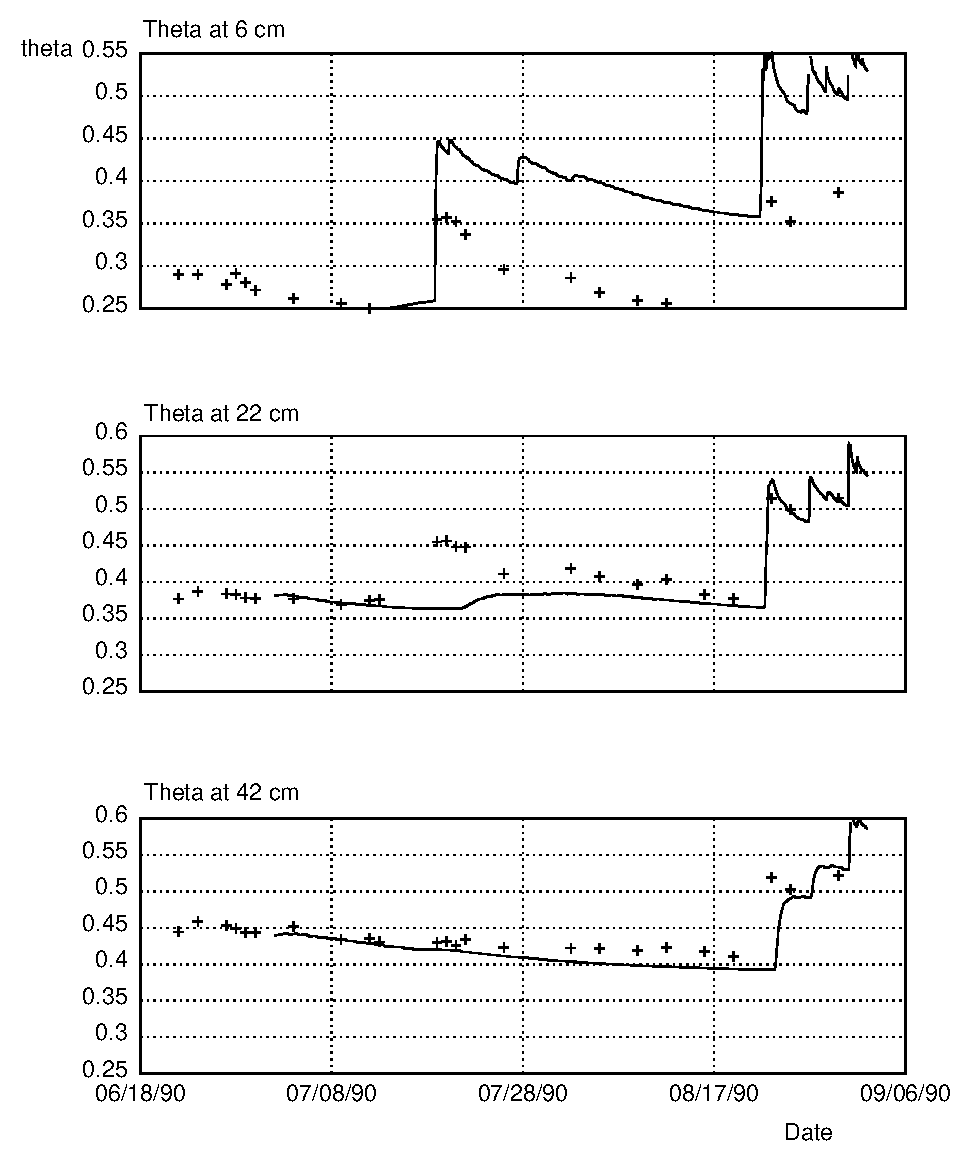
\includegraphics{psfig/mesmod1.eps}
}
\label{fig:mesmodtheta1}
\caption{Measured (plus signs) and modeled (line) water content for layers 
at 6, 22 and 42 cm. below the surface}
\end{figure}

\begin{figure}
\centerline{
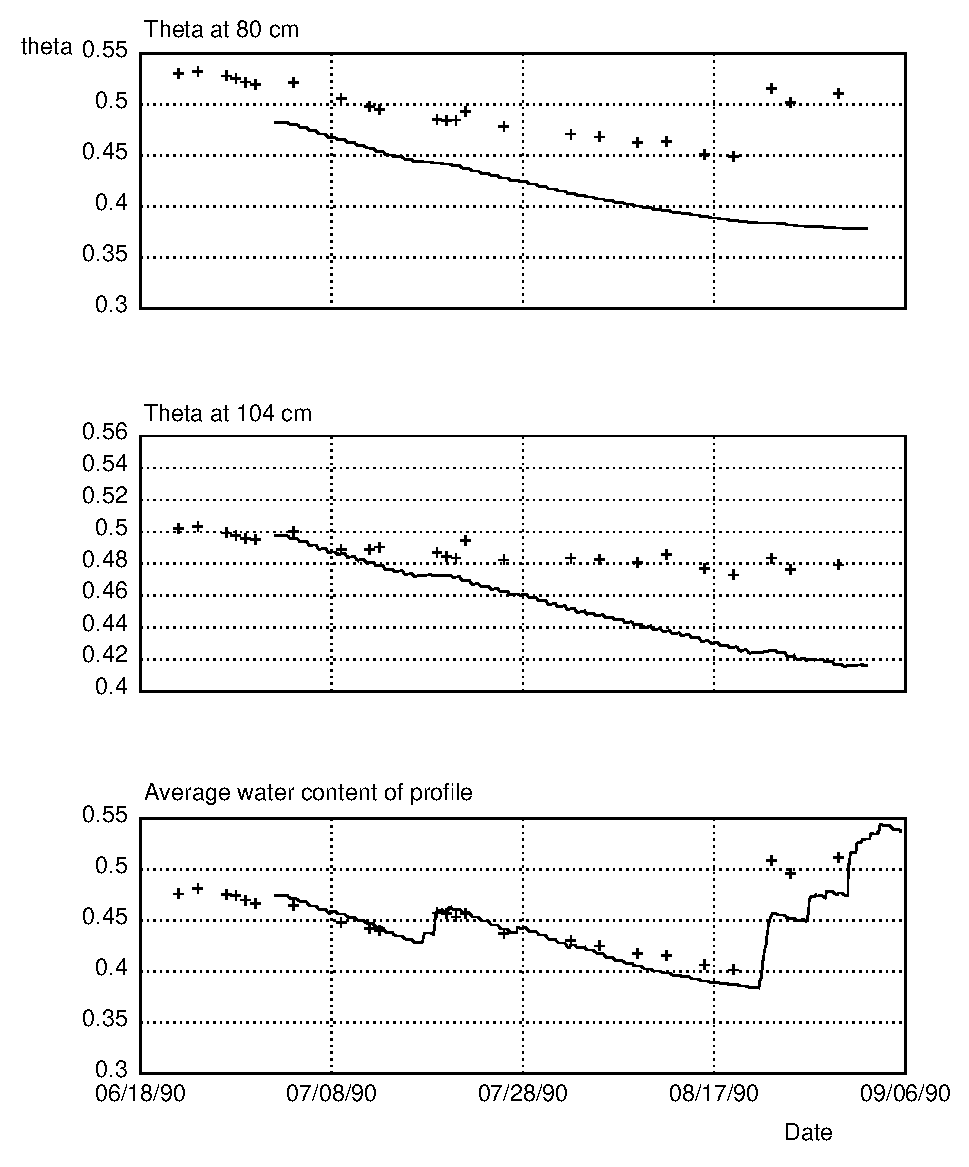
\includegraphics{psfig/mesmod2.eps}
}
\label{fig:mesmodtheta2}
\caption{Measured (plus signs) and modeled (line) water content for layers 
at 80 and 104 cm. The bottom figure shows measured and modeled average water content.}
\end{figure}

\begin{figure}
\centerline{
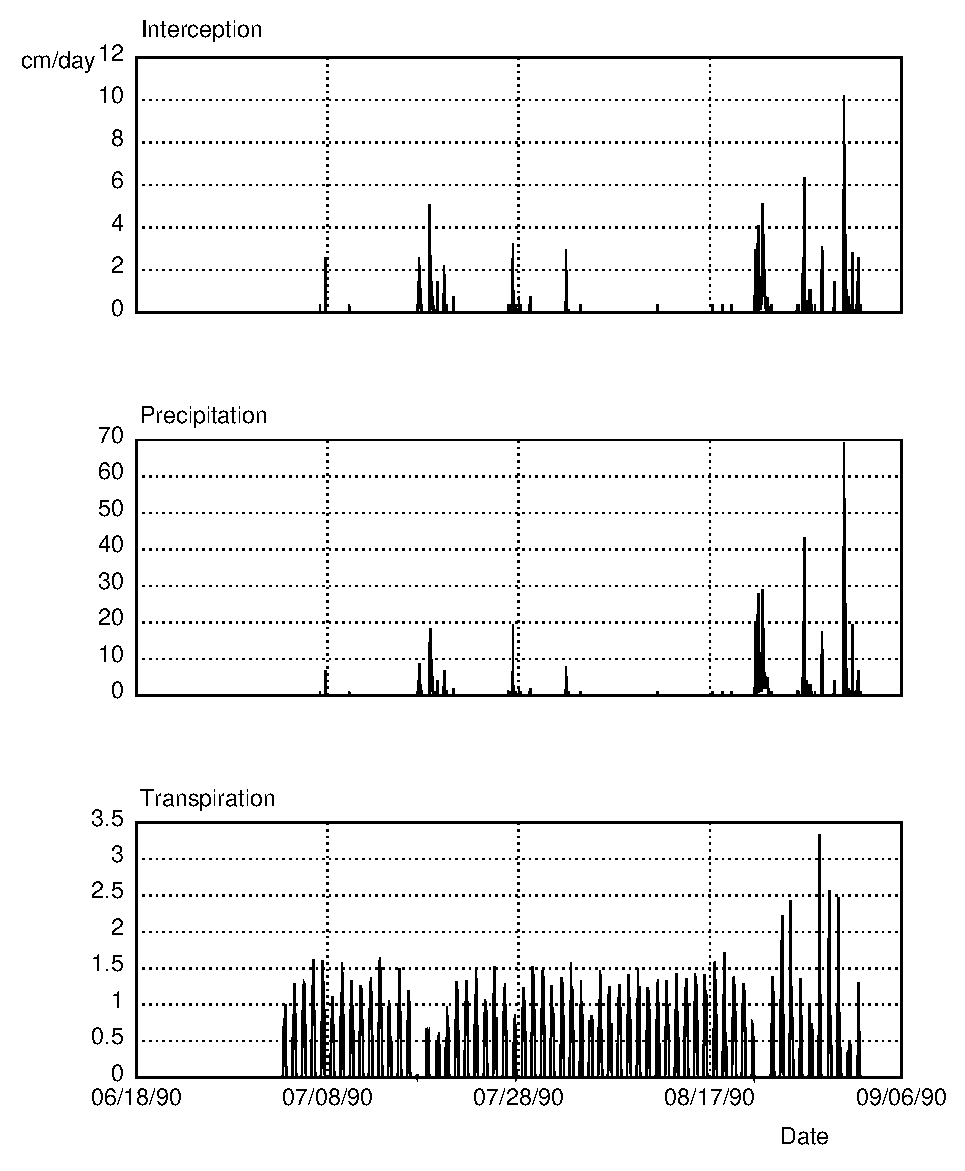
\includegraphics{psfig/watbal1.eps}
}
\label{fig:watbal1}
\caption{}
\end{figure}

\begin{figure}
\centerline{
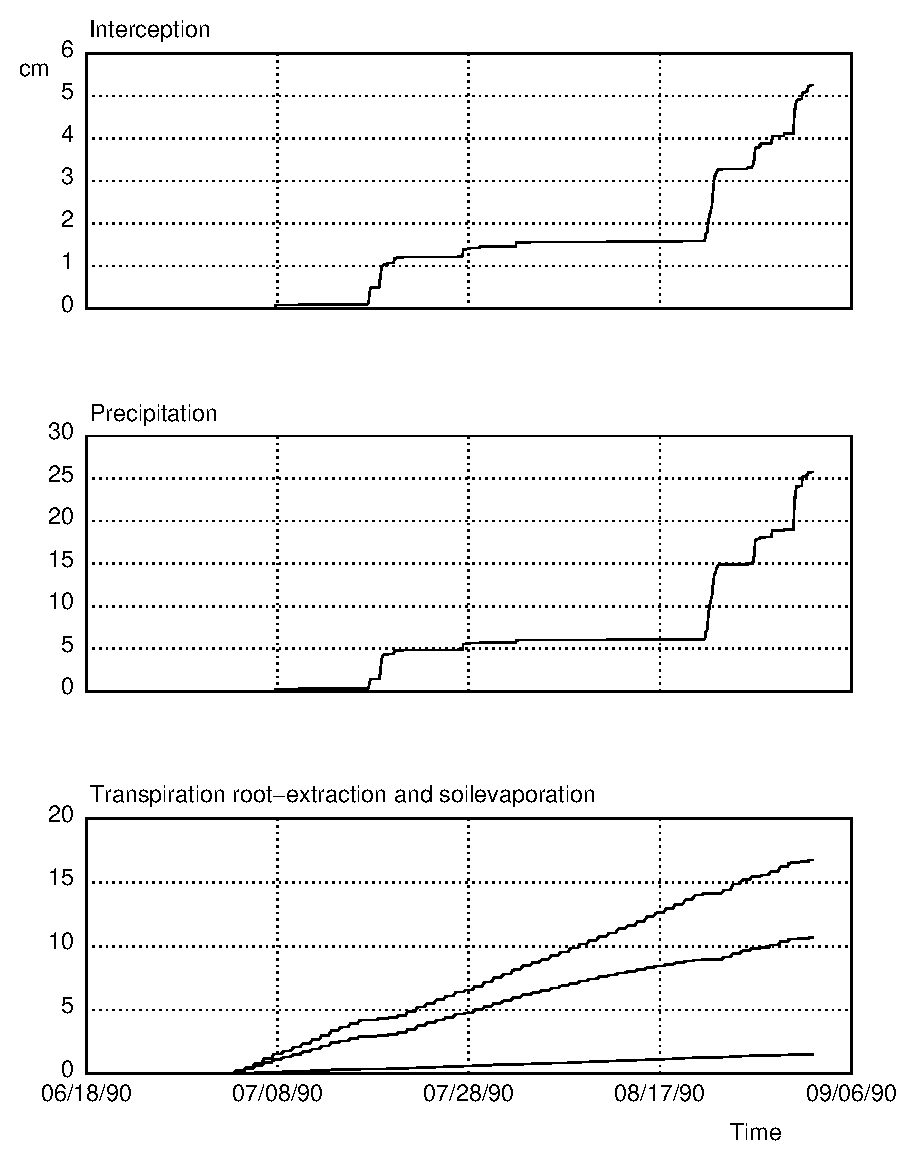
\includegraphics{psfig/watbal2.eps}
}
\label{fig:watbal2}
\caption{}
\end{figure}


\begin{multicols}{2}
{\tiny
\begin{verbatim}
[vamps]
iniinmem=1

[run]
outputfile = run5.hh.out

[determine]
canopy = 1
soilmoisture = 1

[time]
steps = 2930

[ts]
precipitation=../ninp/precip.prn
netrad=../ninp/rnet.prn
rhumid = ../ninp/rh.prn
temp=../ninp/newt.prn
windspeed = ../ninp/wind.prn
sm_probe_avg_theta = ../ninp/theta.mes.ts

[xout]
filename= xout.arn

[interception]
method = 0
# These are pre-cyclone values
E_avg/R = 0.147
p_f = 0.6
p_tr = 0.017
S = 0.08
St = 0.0062

[canopy]
transpiration = 2
Rnet_absorb = 0.975
method = 2
layers = 1
#ra=7.0
z = 12.7
z_0 = 1.5
d = 7.0

[roots]
swsink = 0
swhypr = 0
swupfu = 0
depth = 120.0
hlim1 = -5.0
hlim2u = -50.0
hlim2l = -50.0
hlim3h = -800.0
hlim3l = -1000.0
hlim3 = -1800.0
hlim4 = -12000.0

[soil]
swredu=0
cofred= 0.35
smooth=12
gwlevel = 1.0
outdir = output
pondmx = 0.0
verbose=1
layers= 77
bottom= 6
initprof = 0
theta_initial = 0.200000 0.210000 0.220000 0.220000 0.265000\
0.300000 0.350000 0.375817 0.377095 0.383497\
0.380000 0.380000 0.380000 0.443651 0.400000\
0.400000 0.400000 0.400000 0.410000 0.420000\
0.430000 0.440000 0.470000 0.470000 0.470000\
0.470000 0.470000 0.544194 0.470000 0.470000\
0.460000 0.460000 0.460000 0.460000 0.582024\
0.460000 0.460000 0.460000 0.460000 0.460000\
0.460000 0.514537 0.506907 0.506545 0.505096\
0.504733 0.495707 0.489597 0.492829 0.501117\
0.505820 0.499311 0.497508 0.497508 0.497508\
0.497508 0.497508 0.497508 0.497508 0.497508\
0.497508 0.497508 0.497508 0.497508 0.497508\
0.497508 0.497508 0.497508 0.497508 0.497508\
0.497508 0.497508 0.497508 0.497508 0.497508\
0.497508 0.497508 

# This is from page 70 phd waterloo
# total depth = 2.000000
[layer_0]
description = Tulasewa top layer
thickness=2.000000
theta_initial=0.2
method =1
thetas =0.6
theta_residual = 0.08
thickness = 2.5
alpha = 0.061
n = 1.098
l=0.5
ksat=1800

# total depth = 30.000000
[layer_14]
description = Tulasewa 30 - 75 cm layer
thickness=2.000000
theta_initial=0.4
thetas = 0.64
alpha = 0.042
n = 1.094
l = 0.5
ksat=380.0

# total depth = 74.000000
[layer_36]
description = Tulsewa deep layer > 75 cm
thickness=2.000000
theta_initial=0.46
ksat = 3.0
thetas = 0.6
\end{verbatim}
}
\end{multicols}
